\section{Off-Chaining Data Implementation Strategy}

\begin{itemize}
\item Explain shortly how this approach shall work (maybe reference section 4.3 from Jacobs Paper [\cite{Eberhardt2017}] )
\end{itemize}

\begin{itemize}
\item Figure of our architecture
\item Explanation of systems / subsystems in our architecture
\item How they interact with each other
\item Also, describe which parts are assumed to be trusted
\end{itemize}


\subsection{Architecture}

This section aims to give a broad view of the components and how all of them work together to satisfy the needs of our prototype. A more detailed explanation for each component will be discussed in section \ref{sssec:technologies}.

\begin{figure}[t]%evtl:[t] [!htbp]
\centering
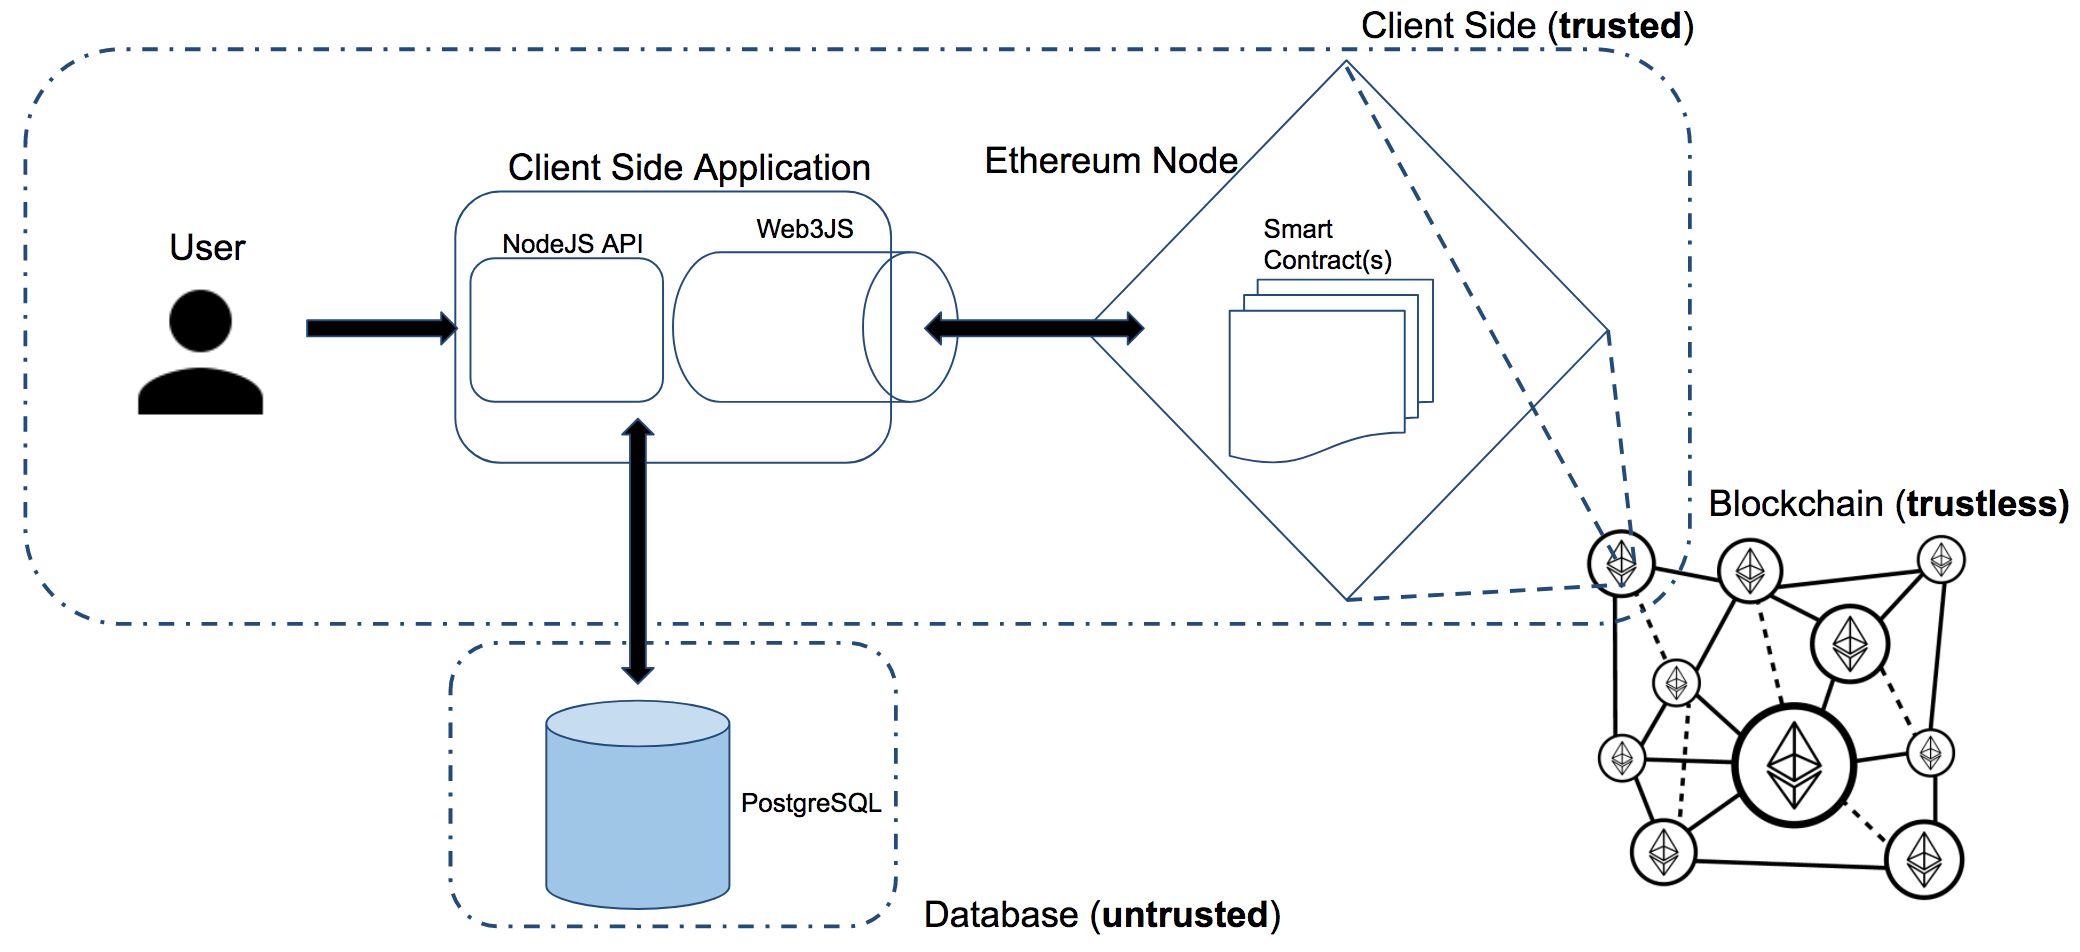
\includegraphics[width=1.0\textwidth]{images/architecture.png}
\caption{\label{fig:architecture}The architecture of the off-chaining approach.}
\end{figure}

As seen in Figure \ref{fig:architecture}, we have divided our architecture into three sides:
\begin{itemize}
\item Client side
\item Database
\item Blockchain environment
\end{itemize}

\subparagraph{Client Side}
The client side consists of the client side application, and the Ethereum node. The client side application is the biggest component as it bridges the database and the smart contract in the Ethereum node. Currently, we put trust into the client side to a certain extent. The extent of trust varies depending on the use case, but nevertheless, a certain level of trust has to exist. For example, upon insertion of new data, before any data goes into the smart contract to be processed, we trust that the client side application will not alter the values. This assumption also acts as a temporary solution to the problem which we have encountered in performing heavy computations inside the smart contract. This assumption has allowed us to take the computational burden from smart contract to the client side application. This problem and solution will be explained in more details in <this section, core implementation stratey>.

\subparagraph{Blockchain Environment}
The blockchain environment is the decentralized network where the smart contract and its local data are going to ultimately live in. The blockchain decentralized network is trustless. But what it truly means is that the trust is distributed amongst all nodes in the network. It also means that we do not enforce an external institution to make sure that the smart contract and its local data are accurate and consistent (integrity). The environment itself ensures the integrity of the data.

\subparagraph{Database}
The database however, is not trusted. Though in our approach we use the database to store data that is going to be used again in the smart contract, we cannot trust the database. The database is prone to internal attacks that can affect the integrity of the data. But at the same time, a database allows us to store large amount of data, and it can be easily integrated with other applications or systems, highly suitable for an off-chaining approach. Hence our approach includes leveraging data integrity check mechanisms when using off-chained data from an untrusted source, such as the database, in the smart contract.

\subparagraph{Transportation Layer}
We have not only made the assumption that our client side is trusted, but also that the transportation layer is secured. Prior to the assumption, we have thought of attacks such as the man-in-the-middle attack, and how detrimental this attack is when we want to save raw data to the database, or when communicating with the smart contract. For example, it could happen that the hashes created in the client side application are altered upon sending them to the smart contract during the initial step. The first step of the approach includes the client side application hashing the raw data and sending the hashes to the smart contract to be stored, mapping the off-chained data to their hashes. Hence, if an attack changes a hash to a different data’s hash, then someone may be able to pass the integrity check by reusing that altered hash’s raw data value.

\subparagraph{Application Flow}
There are two most basic and general approaches in which the user interacts with our client side application. 

\begin{itemize}
\item Inserting a new data
\item Performing a specific action with that data
\end{itemize}

In most general cases, the flow of our application when a user wants to insert a new data goes in the following way: 

\begin{enumerate}
\item User posts a request to client side application with all the data that are required in the specified data model. 
\item Client side application creates a Merkle Tree using the data sent.
\item Client side application sends the Merkle root hash to the the smart contract.
\item smart contract stores the root hash as a local variable.
\item smart contract fires an Event to the client side application to let it know if it has successfully stored it. 
\item Client side application performs a database query to store the data and the root hash into the database.
\item Database stores it.
\item Return success message to the user. 
\end{enumerate}

In most general cases, the flow of our application when a user wants to perform a specific task through the smart contract while using the Off-chained data goes in the following way. 

\begin{enumerate}
\item User creates a request to the client side application to perform a specific smart contract function. 
\item Client side application triggers relevant smart contract function.
\item smart contract triggers an Event to the client side application to retrieve specific data from database. Specific data can be specified by using the root hash stored in smart contract previously.
\item Client side application listens to Event and queries required data from the database.
\item Client side application creates a Merkle tree from the queried data, and creates a Merkle proof.
\item Client side application sends required data and proof to smart contract via function call.
\item smart contract performs integrity check using the proof from client side application.
\item smart contract continues with the original intended task requested by the user when the proof has passed the integrity check. 
\item smart contract computes a new root hash from the new changed value, and stores it.
\item smart contract triggers an Event back to the client side application containing either the results, or an error when the proof does not satisfy the condition of the integrity check. 
\item Client side application listens to Event stores the new root hash and the new changed value into the database. 
\item Client side application finally returns either a success message, or a failure in case of a failed data integrity check. 
\end{enumerate}

\subsection{Technologies}


\subsubsection{Smart Contracts, Solidity Truffle and Ganache}

\subparagraph{Smart Contracts} 
Computer programs that are executed automatically when conditions (terms) of the contract have been met. Understanding smart contracts in a high-level aspect are the same as standard contracts. While a standard contract enforces the terms of a contract (regularly by law), a smart contract actualizes this enforcement of terms through network consensus and cryptography. These programs are executed in a trustless and carefully designed way in the network and are referred as Smart Contracts. Ethereum is one of the most known platforms, it empowers developers to create their own smart contracts and creating decentralized applications in the blockchain. Upon creation of smart contracts, they need to be executed in a secured runtime environment. Therefore, the creation of Ethereum Virtual Machine (EVM) is the runtime for Smart Contracts. Putting it in simpler understanding, EVM is a virtual machine that continues running on every node in the system/network and executes smart contracts. In addition, it is isolated that no framework or filesystem access is possible, thus to ensure determinism. Moreover, to be able to use Smart Contracts, higher level programming languages which compile EVM code have been developed such as Solidity, Serpent, LLL [citation]

\subparagraph{Solidity}
Being as one of the most used contract-oriented high-level programming language for executing smart contracts. It was inspired by C++, Python, and JavaScript and is intended to focus on the Ethereum Virtual Machine (EVM). Solidity is compiled to bytecode that is executable on the EVM. Through Solidity, developers can write applications that enable self-enforcing business rationale exemplified in smart contracts, leaving an unchangeable and definitive record of transactions. Solidity is a statically typed, which inheritance is supported, libraries and complex user characterized types among other features.[citation]

\subparagraph{Truffle}
The most popular development framework for Ethereum. It is written in JavaScript, therefore, being more flexible and providing numerous built-in features that assist and make the development easier. Truffle aims to handle the process of compilation, linking, deployment and binary management of smart contracts. Furthermore, it supports network management for deployment to private and public networks, its interactive console – which provides access to your built-in contracts, and availability of having automated contract testing through Mocha and Chai JavaScript test framework. In the scope of this project, we decided to start our implementation in Truffle framework. One of the main reason was due to the advantage of Truffle having a wider and active community support and availability of online resources, than any other Ethereum development frameworks. Moreover, the possibility of truffle integration with NodeJS became an important and crucial advantage for our implementation due to our team’s advanced skills on JavaScript. [citation] programming.

\subparagraph{Ganache}
It originates from the former known TestRPC,  which was a local (virtual) Ethereum blockchain for development purposes. It simulates the blockchain network, allowing you to make RPC calls in it without the need of actually mining the blocks. Ganache was developed by Truffle and is included in their latest development in Truffle Suite. The release of Ganache was positively anticipated across the whole Truffle framework, specifically in performance aspects - being much faster. Moreover, a huge advantage was providing an interface to the developer with the details of all the transactions being mined and their costs which further improved the user experience of the whole development platform itself [citation]


\subsubsection{Node.js, Express and Web3.js}

\subparagraph{Node.js}
Being an open source cross-platform based on Chrome's JavaScript runtime for effortlessly constructing quick, scalable applications. Node.js utilizes an event driven, non-blocking I/O model which that makes it lightweight and effective, ideal for data-intensive real-time applications that keep running throughout distributed devices. Through event-driven property, meaning that the server reacts at the time when an event occurs therefore allowing us to create easily scalable, fast and real-time applications.[citation]

\subparagraph{Express}

Being a project from a node.js foundation, which is a quick, moderate web application framework for Node.js. It is intended for building web applications and is the true standard server system for Node.js. In the scope of our project we use Express as a basic routing layer built over the base of Node.js HTTP server that manages a server and the routes. It gives declarative routing without the need of doing “switch” or “if” statements or any additional functions, into a fundamental middleware design. [citation]

\subparagraph{Web3.js}
An aggregation of libraries which contain specific functionality for the ethereum environment and enables you to interact with a local or remote ethereum node, utilizing a HTTP or IPC connection [citation]



\subsubsection{PostgreSQL and Sequelize}
\subparagraph{PostgreSQL}
An open source and highly scalable object-relational database system, which runs on all major operating systems including Linux, UNIX (AIX, BSD, HP-UX, macOS, Solaris), and Windows. It is completely ACID obedient, has full assistance for foreign keys, joins, views, triggers. [citation]

\subparagraph{Sequelize}
A promise-based Node.js ORM for PostgreSQL, MySQL, SQLite and Microsoft SQL Server. It highlights strong transaction support, relations, read replication etc. [citation]


\subsubsection{Build-up/ Deployment Tools}
\subparagraph{Docker}
A deployment tool intended to make it less demanding to create, deploy, and run applications by using containers. Containers enable a developer to bundle up an application with all the parts it needs, such as libraries and different dependencies, and deliver everything out as one package. Thusly, because of the container, the developer can be certain that the application will run the same way on other machines, independently of their different operating system or any customized settings that the other machine may have. This gives a huge performance boost and decreases the extent and the size of the applications itself. [citation]

\subsection{Use Cases}

\subsubsection{Proof of Concept: Counters}

Here goes my text.

\paragraph{Introduction}
In companies large amounts of data records are retrieved and modified each day. But what if data records are changed or manipulated in a way that the results of your calculations with the data become wrong and decisions are made based on these results? Guaranteeing the integrity of data records in a distributed environment is a big challenge.

This challenge can be tackled by using blockchain technologies. Storing data in the blockchain can guarantee the integrity of your data at all time. Although it gives you many other advantages, storing data, especially large amounts of data, on the blockchain can be very expensive.

The task of this project is to find ways to guarantee the integrity of data stored in a RDBMS with the help of smart contracts. The general idea is to perform integrity checks on data in the smart contract, whenever data is required to perform any transaction. For the current project stage two uses cases have to be found and developed. The use cases shall show the potential benefit of storing large amounts of data off-chain but still being able to guarantee the integrity of the data. This is always the case when it comes to financial or personal/contract data.

In the first step specific requirements for the uses cases have to be formulated. For the first use cases very complex examples may not be feasible at this project stage. The idea is to generate simple uses cases first, apply these to the current prototype implementation, test them in terms of performance and efficiency and show ways to further develop the use cases as well as apply different integrity mechanisms based on the results of the tests.

In the second part, two different use cases are presented, which were developed during discussions with the project team. The uses cases should represent a real case scenario and highlight the need for off-chaining data.

\paragraph{Requirements}
The following points should summarize the requirements for the first use cases. As mentioned before, the developed uses cases should still be feasible and integratable with the current prototype implementation. Also too complex examples might lead to reaching the resource limit (gas limit) quickly without having implemented efficient integrity mechanisms.

\begin{itemize}
\item Multiple Columns:
In order to make use of the hash tree algorithm a data table with multiple columns is required.
\item One table per Use Case:
In the current project stage, the Use Cases should use only one table each. Multiple entities and relations would make the Use Case too complex. At further project stages a more complex Use Case with multiple entities and relations could be developed.
\item Big Data:
In real world examples large numbers of data records are stored and evaluated every day. Our use cases should consider real world examples, where a large amount of data is required. With the current prototype implementation and the posed constraints by the Ethereum network, a large number of data records could hit the gas limit very quickly. Therefore, the number of data records should be limited to a defined number.
\item Different Scenarios:
For presentation purposes, the two use cases should not only use different data types but also do different things with the acquired data. For now we agreed on two different scenarios: 1. Check only (integrity check) and 2. Check and Modify (also update data).
\end{itemize}

In the next chapters, we will discuss the two different scenarios and the specific use case for each scenario.

\paragraph{Scenarios - Use Cases}
In the overall scenario, we assume that the smart contract requires data in order to perform a task and a transaction. The main operation of the smart contract should be the integrity check of the acquired data from the RDBMS. A possible scenario can stop at this point, where the smart contract only returns the result of the integrity check. A more advanced scenario would be that the data has to be modified by a smart contract function. In conclusion for this task these two scenarios should cover our use cases:


\subsubsection{Employee Use Case}
\paragraph{Scenario 2: Check and Modify}
Generic Steps:
\begin{itemize}
\item Client sends request to Client-Side Middleware to perform an action/ a transaction
\item Client-Side Middleware triggers relevant Smart Contract function
\item Smart Contract triggers Event to retrieve specific data
\item Client-Side Middleware listens to Event and queries required data from the database
\item Client-Side Middleware sends required data to smart contract via function call
\item Smart Contract checks integrity
\item Smart Contract modifies data (and computes new Merkle tree)
\item Smart Contract triggers Event to send modified data (and new Merkle tree)
\item Client-Side Middleware listens to Event and stores modified data and Merkle tree to database
\end{itemize}

\paragraph{Concept - Employee Payraise}
Description
A company and a union agreed on a specific salary raise (%) for employees in a specific department and specific entry date. The salary raise (%) is stated in a smart contract. The current salaries of the affected employees have to be verified before the raise can be applied.

Table missing: gDoc "Use Cases for Off-Chaining Data"

In a first implementation, the Smart Contract stores the root hash of the table entry for each employee with the current salary plus the root hash of the table row with the previous salary. Like this, we can calculate the salary raise on-chain as well if needed.
The hash of the ID and the hash of the salary should be calculated on-chain while the other columns per record can be hashed in the middleware and provided to the Smart Contract. Only the hash over all the column hashes has to be stored on the blockchain. Therefore, it is certain that the ID of an employee and the corresponding salary cannot be pushed into the blockchain in a wrong way and later on updating the salary for a different employee.

With this approach it can be verified that an employee with a distinct ID is earning a certain salary now and earned a certain salary before that. In addition, the current salary can be updated to represent current negotiations or promotions. A third party like a union could verify that the salary is updated correctly and point to the record on the blockchain in case of conflicts. The contract could e.g. be queried to return the verified salary for a given employee ID or return the IDs of employees for a given salary.

At the same time privacy is given here (as an additional benefit) because the Smart Contract never stores the employee’s ID or the salary (only the two root hashes).


\paragraph{Implementation}

\subsubsection{Financials Use Case}
\paragraph{Scenario 1: Check only}
\subparagraph{Generic Steps - Event Based:}
\begin{itemize}
\item Client sends request to Client-Side Middleware to verify specific data (data or indexes are not known by Client)
\item Client-Side Middleware triggers relevant Smart Contract function
\item Smart Contract triggers Event to retrieve specific data
\item Client-Side Middleware listens to Event and queries required data from the database
\item Client-Side Middleware sends required data to smart contract via function call
\item Smart Contract checks integrity
\item Smart Contract triggers Event to send result of integrity check (result = corrupted records or true/false)
\item Client-Side Middleware listens to Event and sends the result back to client
\end{itemize}

\subparagraph{Generic Steps - Data to check is Known:}
\begin{itemize}
\item Client sends request to Client-Side Middleware to verify specific data (data or indexes are not known by Client)
\item Client-Side Middleware queries required data from the database
\item Client-Side Middleware sends required data to smart contract via function call
\item Smart Contract checks integrity
\item Smart Contract triggers Event to send result of integrity check (result = corrupted records or true/false)
\item Client-Side Middleware listens to Event and sends the result back to client
\end{itemize}

\paragraph{Concept - Financials}
\subparagraph{Description}
An external auditor wants to check the financial situation of a company. One task could be to check the stated weekly or monthly sales amount against the sum of all sales records in the specific year. One of the first steps would be to verify (check the integrity) of all sales records in the specific year.

This use case consists of two parties, a financial auditor and the company that holds the financial data. An assumption that we make is that the middleware is open-sourced, produced by an auditing company, and it is being consumed by the company to store their financial data in the Blockchain environment. The middleware allows the company to off-chain their financial records from the Smart Contract into a database, while maintaining the integrity of the data using the Blockchain environment. The middleware also allows the auditor to easily audit companies’ financial records without having to worry about the integrity of data once they are appended. It also allows the auditor to query the financial records with a filter, such as the date of the records, performing query completeness. The middleware however does not allow users to edit the records through the middleware, though it is possible to do it on the database directly, which will then result in an integrity check error when the records are used or verified by the auditor. 

\textit{Example: A Sales Table}
\begin{center}
    \begin{tabular}{| l | l | l | l | l |}
    \hline
    ID & Product & Date & Amount & Price \\ \hline
    1 & Wallet & 20171230 & 1 & 20 \\ \hline
    .. & ... & .... & .. & ... \\ \hline
    \end{tabular}
\end{center}

The different table rows represent moments in time (e.g. every Friday night after 00:00 or every first of the month) and thus new records are appended to the table. In this way, the records can be tracked back in time and an auditor could double-check the records for e.g. the last 6 months or the last 104 weeks. The Smart Contract entry then consists of the root hash over every table row (with each column being a leaf in the Merkle tree).

As the database is under the control of the company storing their financial figures, the financial auditor cannot be sure that those numbers were inserted correctly (same as without blockchain). By having the hashes of the records on the blockchain, the auditor can be sure that the company was not able to change the figures later on and thus has the certainty that there are no accounting tricks and malpractices in place e.g. at the end of the year or quarter. The figures that were once recorded by the company can be double-checked afterwards (or it can be noticed that the company recorded wrong numbers or tried to change them in hindsight). It is worth mentioning that the Smart Contract never stores the financial figures and they are thus not available on the blockchain either. While upon insertion, there isn’t a way to check that the numbers are true, but we can assert that these numbers will not be prone to illegitimate changes. 

Furthermore, this use case could be valuable for rewarding benefits to employees. For example, the CEO of a company could receive a benefit by the shareholders (indirectly through the company itself but signed by the shareholders) if certain financial data are met. Or a sales person in the company could receive a benefit for sales data records for a certain month that went especially well. 

To conclude, this use case asserts that large quantities of data (like financial figures of a company) cannot be modified after reporting them while only storing a relatively cheap representation of that data (hash) on the blockchain. Third parties and internal controllers are thus able to rely on the integrity of the recorded data. 

\paragraph{Implementation - Financials}
\subparagraph{Initial Concept: Whole Table Verification}

In this initial approach and concept, we created an assumption that the financial rows are prone to changes, and that the Smart Contract is going to keep track of the total or the aggregation of the rows. Hence, a verification of the whole table is needed to ultimately maintain the integrity of the “Total” row.

The Smart Contract stores the current root hash of the whole table. It could also store the root hashes of the prior states of the table (this info could otherwise be found in the blockchain history) to allow for additional functionalities.

The Smart Contract creates a Merkle tree over the hashes of all rows. The hashes of the rows are provided by the middleware. Afterwards, the Smart Contract verifies that the root hash of the created Merkle tree matches the stored current root hash. If that is the case, it calculates the new total value(s), and adds the hash of the new row (new entry) to the Tree to create the new root hash after these processes. This new root hash is then stored as the current one. 

Merkle tree is used here when a column, or multiple column values are changed in a row, and we need to recalculate the new values for the Total row. Instead of verifying the whole data in a row, we only need to verify the nodes that are affected by the change. 

For the Merkle tree implementation, there is no need to implement a new one or change the existing one, as we can use the Multiple Item Proof here (note: an item here will correspond to a row, not a column).

Append row - Steps:
\begin{enumerate}
\item First, the client side application gets all the data from the Database.
\item It then creates the proof and sends it to the Smart Contract.
\item The Smart Contract does the integrity check. 
\item Now, first the new total values are calculated, the Smart Contract 
\item creates a root hash for that total row, then recreates the tree with 
\item that new roothash from the total row, and that newly added item row. 
\item Send back the total row, and that newly added item row. 
\end{enumerate}

\subparagraph{Realization}

We quickly realized the “red flags” this approach is producing in regards to the gas cost. In the process of adding a new row, we are adding a new leaf, or a new hash into the current Merkle tree (step 4), and this does not work that way, as we are planning on having only the Merkle proof, the nodes that are not affected by the change. Hence, to approach this we always have to send all of the leaves, the hashes of the rows, so that we can create this new tree in addition to a new leaf, the new hash of the inserted row. This quickly creates an overhead in the gas cost when adding a new row into the table. Hence, we took a turn in our approach, and we have to come up with something more usable, and worth it for the users. While the same gas cost problem will still exist in the next approach, it will however provide a much larger incentive for using the function. 

\subparagraph{Query Completeness}

Query completeness is the concept that we came up with that can better leverage the whole table verification. Furthermore, it addresses an important real-world problem. A user queries the database, however, does not want to put trust into the returned results. The blockchain can be used as an objective verifier of the query results. See section \ref{sssec: queryCompleteness} to learn more about the concept. An example on how this mechanism is applied to our use case includes a user who wants to query all sales data in the period from Nov 2017 to Jan 2018, and expects that the results have not been tampered with. 


Initial implementation idea:
\begin{itemize}
\item Verify that all entries were considered and that none were left out in the returned results.
→  have database respond to original query and to the negated query (e.g. original: all sales data in the period from Nov 2017 to Jan 2018, negated: all sales data NOT in the period from Nov 2017 to Jan 2018)
→ check that combined size of both returned lists equals total number of entries (mapping counter in SC)
\item Verify that only actual entries from the database were returned
→ combine the two result lists to one Merkle proof to show that all rows are part of the table, i.e. no entries were changed and no outside entries were returned as a result
\item Verify that the returned results match the query requirements (are “correct”)
→ no feasible way with blockchain currently as we would either need to do a lot of computation or to store a large amount of data (maybe even all data) on-chain, which would contradict this project’s focus
→ leave this verification up to the user (she can see whether the results match her query)
\item Verify that all results that match the query were actually returned
→ no feasible way with blockchain currently as we would either need to do a lot of computation or to store a large amount of data (possibly even all data) on-chain, which would contradict this project’s focus
→ unfortunately, the user does not have an easy way to verify that either
\end{itemize}

The above statements show that there is a clear trade-off between achieving Query Completeness and this project’s goal of saving gas costs by off-chaining data. Either practically all data has to be stored on-chain to enable our smart contract to guarantee Query Completeness, or a plethora of computations (Merkle proofs for each row in the data table) have to be on-chained which would hit the gas limit relatively fast. 

As we are facing the challenge described previously, we decided to implement our proof of concept for Query Completeness by adding assumptions to make it feasible and easier for testing for large amount of data: building on our initial assumption that we trust our client-side application, we calculate the Merkle proofs on the client-side and thus save a considerable amount of computation on-chain. Nevertheless, the smart contract will check the integrity of the data and perform a simplified query to guarantee Query Completeness. We also only allow the Date column to be used in the query in this proof of concept

\subparagraph{Proof of Concept}

This section describes the step-by-step actions between our client-side application, Smart Contract and the Database. The proof of concept includes the implementation of appending a new financial row, and query completeness. We want to remind the readers to keep in mind the previous assumptions that we have stated. 


\textit{Example: This table shows how the records are stored in the database, assuming all data here are appended through the Smart Contract.}
\begin{center}
    \begin{tabular}{| l | l | l | l | l | l | l | l |}
    \hline
    ID & company\_name & roothash & total\_sales & date & cogs & sc\_id & ... \\ \hline
    1 & CompanyAB & 0x123 & 1000 & 20160523 & 123 & 0 & .. \\ \hline
    2 & CompanyAB & 0x134 & 2000 & 20161215 & 421 & 1 & .. \\ \hline
    3 & CompanyAB & 0x321 & 3000 & 20170601 & 222 & 2 & .. \\ \hline
    4 & CompanyAB & 0x789 & 9000 & 20180130 & 980 & 3 & .. \\ \hline
    \end{tabular}
\end{center}



\textbf{\textit{Appending A Finanical Row}}

\begin{figure}[h]%evtl:[t] [!htbp]
\centering
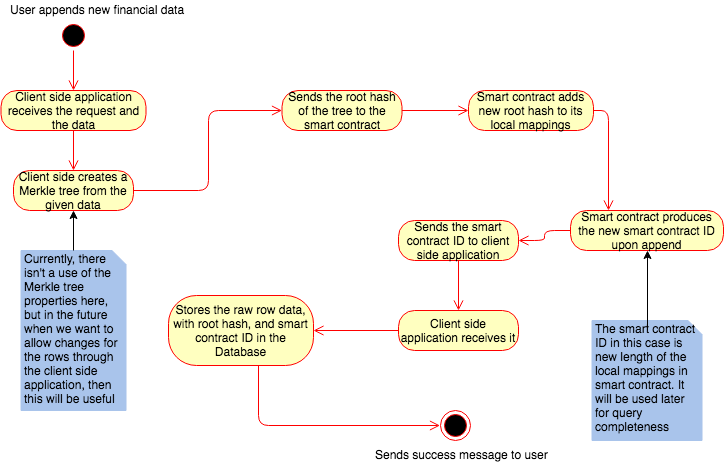
\includegraphics[width=1.0\textwidth]{images/appendRowFinancials.png}
\caption{\label{fig:appendRowFinancials}Activity diagram of appending a row to the financials record}
\end{figure}

\begin{enumerate}
\item User appends a new financial data, providing all the required information to be in the database
\item Client-side application then creates a Merkle tree from the given raw data
\item Sends the root hash of the created Merkle tree to the Smart Contract 
\item Smart Contract appends that new root hash into its local mappings. 
\item Smart Contract increments the new length of the mapping, which is the Smart Contract ID that is going to be returned. This acts as an identifier to which hash belongs to which financial row. It is also used to preserve the ordering of the hashes which will later be used for Query Completeness. 
\item Smart Contract sends back the Smart Contract ID to the client-side application
\item Client-side application saves the raw financial data, with the root hash, and the Smart Contract ID. 
\end{enumerate}

\textbf{\textit{Query Completeness}}

\begin{figure}[h]%evtl:[t] [!htbp]
\centering
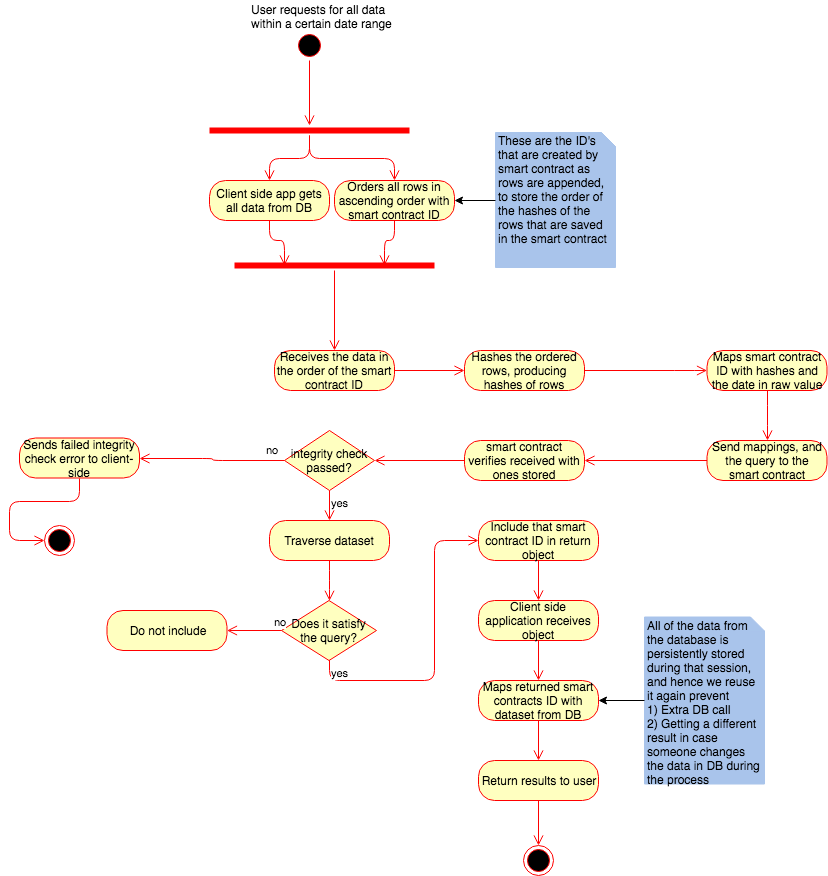
\includegraphics[width=1.0\textwidth]{images/queryCompleteness.png}
\caption{\label{fig:queryCompleteness}Activity diagram for query completeness}
\end{figure}


\begin{enumerate}
\item User requests to get all of financial data that are within the data range the user has requested.
\item The client-side application gets all data from the database in the ascending order of the Smart Contract ID. This ID is generated by the Smart Contract to keep the ordering of the hashes that are stored in the Smart Contract. It is generated upon appending a financial record through the Smart Contract. 
\item The client-side application hashes all the returned rows
\item It will then maps the hashes of the row and the raw date value to the Smart Contract ID.  
\item The client-side application sends the mapping with the query to the Smart Contract.
\item The smart contract checks if it got the right data, the right amount of rows and the correct table overall by iterating over the provided root hashes and comparing them to the previously stored ones.
	\begin{enumerate}
	\item If Smart Contract cannot verify the rows, then it will throw an integrity check error to the client-side application as an event. 
	\item If the smart contract can confirm this, it checks the query condition for every row and returns (better: puts into an event) an array of booleans indicating all the indexes of rows that fulfill the query. Dates are intentionally stored as “uint” to ease the query function in the smart contract. For example 1, March, 2018 -> 20180301
	\end{enumerate}
\item Smart Contract returns back all the Smart Contract IDs that have satisfied the query.
\item The client-side application listens to this event and returns the specified rows to the user subsequently.
\end{enumerate}





\subsection{Translator}

Manually integrating off-chaining into an existing smart contract which uses state variables (on-chained contract) requires advanced knowledge of the implementation of both the given contract and our integrity check mechanism. This inevitably introduces a barrier to potential users as they have to familiarize themselves with implementational details of our solution. Moreover, it prevents use cases where knowledge about the implementation of a contract cannot be obtained with reasonable effort, e.g., in the case of automatically generated contracts. Since translating an on-chained contract into an off-chained one is a static procedure, we decided to develop a proof-of-concept of a program which automates this process, referred to as \emph{translator}, to make off-chaining accessible and easy to use.

The functionality of the translator can be divided into the following steps:
\begin{enumerate}
\setlength{\itemsep}{0pt}
\setlength{\parskip}{0pt}
	\item Check given contract
	\item Parse contract, variables and functions
	\item Determine off-chained values
	\item Render off-chained values to templates
	\item Copy static files.
\end{enumerate}
After the validity of a given contract was checked, the contract is parsed to determine the individual state variables and functions. Each state variable is split up into its name, type, size (in the case of an array), and the original descriptor string, which describes the variable in the smart contract. Subsequently, each function is parsed to determine which state variables are used and which are modified. A function's original arguments and modifiers are parsed as well since they also need to be included in the off-chained version of the respective function. After the contract was decomposed into the individual data structures (contract, variables, and functions), the required values for the off-chained version of the given contract are computed. These values comprise the names and arguments of the respective functions and events of the off-chained contract in several required formats. The resulting values are then rendered into templates to produce the off-chained contract and the corresponding client-side application. In the last step, all resources which do not depend on the content of the given contract are simply copied to the previously specified output location.

The translator's current state of implementation suffices to proof the suitability of the described translation approach. Nevertheless, it has to be further developed to a stable state until it could be applied to real use cases. This particularly includes the automated assessment and validation of a given smart contract, as some variable types and functional structures are not suitable for off-chaining,\footnote{Mappings are an example of an unsuitable variable type, as the Solidity language specification prevents their use as function arguments. Private functions which alter state variables are among the functional structures which are hard to off-chain in an automated manner since the off-chained function must be called from outside the smart contract to pass the off-chained variables.} which at this point still depends on domain knowledge.
